
\normalsize

\section{Formal Definitions}

In this section, we formally define HAT transactional semantics. Our
formalism is based off of that of Adya~\cite{adya}. For the reader
familiar with his formalism, this is a mostly-straightforward exercise
combining transactional models with distributed systems
semantics. While the novel aspects of this work largely pertain
to \textit{using} these definitions (e.g., in Section~\ref{sec:hats}),
we believe it is instructive to accompany them by appropriate
definitions to both eliminate any ambiguity in prose and for the
enjoyment of more theoretically-inclined readers.

\subsection{Model}

Here, we briefly describe our database model. It is, with the
exception of sessions, identical to that of Adya~\cite{adya}. We omit
a full duplication of his formalism here but highlight several salient
criteria. We refer the interested reader to Adya's Ph.D. thesis,
Section 3.1 (pp. 33--43).

Users submit transactions to a database system that contains multiple
versions of sets of objects. Each transaction is composed of writes,
which create new versions of an object, and reads, which return a
written version or the initial version of the object. A transaction's
last operation is either \texttt{commit} or \texttt{abort}, and there
is exactly one invocation of either these two operations per
transaction. Transactions can either read individual items or read
based on predicates, or logical ranges of data items.

\begin{definition}[Version set of a predicate-based operation]
When a transaction executes a read or write based on a predicate P,
the system selects a version for each tuple in P’s relations. The set
of selected versions is called the \textit{Version set} of this predicate-based
operation and is denoted by Vset(P).
\end{definition}

A history over transactions has two parts: a partial order of events
reflects the ordering of operations with respect to each transaction
and a (total) version order ($\ll$) on the committed versions of each
object.

As a departure from Adya's formalism, to capture the use of session
guarantees, we allow transactions to be grouped into sessions. We
represent sessions as a partial ordering on committed transactions
such that each transaction in the history appears in at most one
session.

\subsection{Conflict and Serialization Graphs}

To reason about isolation anomalies, we use Adya's concept of a
conflict graph, which is composed of dependencies between
transaction. The definitions in this section are directly from Adya,
with two difference. First, we expand Adya's formalism to deal
with \textit{per-item} dependencies. Second, we define session
dependencies (Definitions~\ref{def:sd1} and~\ref{def:sd2}).

\begin{definition}[Change the Matches of a Predicate-Based Read]
A transaction $T_i$ changes the matches
of a predicate-based read $r_j$(P:Vset(P)) if $T_i$ installs $x_i$, $x_h$
immediately precedes $x_i$ in the version order, and $x_h$ matches
P whereas $x_i$ does not or vice-versa. In this case, we also
say that $x_i$ changes the matches of the predicate-based read.
The above definition identifies $T_i$ to be a transaction where
a change occurs for the matched set of $r_j$ (P: Vset(P)).
\end{definition}

\begin{definition}[Directly Read-Depends]
$T_j$ directly read-depends on transaction $T_i$ if it directly
item-read-depends or directly predicate-read-depends on $T_i$.
\end{definition}

\begin{definition}[Directly item-read-depends by $x$]
$T_j$ directly item-read-depends on transaction $T_i$ if $T_i$ installs some
  object version $x_i$ and $T_j$ reads $x_i$.
\end{definition}

\begin{definition}[Directly item-read-depends]
$T_j$ directly item-read-depends on transaction $T_i$ if $T_j$
  directly item-read-depends by $x$ on $T_i$ for some data item $x$.
\end{definition}

\begin{definition}[Directly predicate-read-depends by $P$]
Transaction $T_j$ directly predicate-read-depends by $P$ on
transaction $T_i$ if $T_j$ performs an operation $r_j$(P: Vset(P)),
$x_k$ $\in$ Vset(P), $i = k$ or $x_i \ll x_k$ , and $x_i$ changes the
matches of $r_j$ (P: Vset(P)).
\end{definition}

\begin{definition}[Directly predicate-read-depends]
$T_j$ directly predicate-read-depends on $T_i$ if $T_j$ directly
  predicate-read-depends by $P$ on $T_i$ for some predicate $P$.
\end{definition}

\begin{definition}[Directly Anti-Depends]
Transaction $T_j$ directly anti-depends on transaction $T_i$ if it
directly item-anti-depends or directly predicate-anti-depends on
$T_i$.
\end{definition}

\begin{definition}[Directly item-anti-depends by $x$]
$T_j$ directly item-anti-depends by $x$ on transaction $T_i$ if $T_i$
  reads some object version $x_k$ and $T_j$ installs $x$'s next
  version (after $x_k$) in the version order. Note that the
  transaction that wrote the later version directly item-anti-depends
  on the transaction that read the earlier version.
\end{definition}

\begin{definition}[Directly item-anti-depends]
$T_j$ directly item-anti-depends on transaction $T_i$ if $T_j$
  directly item-anti-depends on transaction $T_i$.
\end{definition}

\begin{definition}[Directly predicate-anti-depends by $P$]
$T_j$ directly predicate-anti-depends by $P$ on transaction $T_i$ if
  $T_j$ overwrites an operation $r_i(P:$ Vset(P)). That is, if $T_j$
  installs a later version of some object that changes the matches of
  a predicate based read performed by $T_i$.
\end{definition}

\begin{definition}[Directly predicate-anti-depends by $P$]
$T_j$ directly predicate-anti-depends on transaction $T_i$ if $T_j$
  directly predicate anti-depends by $P$ on $T_i$ for some predicate
  $P$.
\end{definition}

\begin{definition}[Directly Write-Depends by $x$]
A transaction $T_j$ directly write-depends by $x$ on transaction $T_i$
if $T_i$ installs a version $x_i$ and $T_j$ installs $x$'s next
version (after $x_i$) in the version order.
\end{definition}

\begin{definition}[Directly Write-Depends]
A transaction $T_j$ directly write-depends on transaction $T_i$ if
$T_i$ directly write-depends by $x$ on $T_j$ for some item $x$.
\end{definition}

\begin{definition}[Directly Session-Depends by $S$]
\label{def:sd1}
A transaction $T_j$ directly session-depends on transaction $T_i$ if
$T_i$ immediately precedes $T_j$ in the session commit order for session $S$.
\end{definition}

\begin{definition}[Directly Session-Depends]
\label{def:sd2}
A transaction $T_j$ directly session-depends on transaction $T_i$ if
$T_j$ directly session-depends on transaction $T_i$ for some session
$S$.
\end{definition}

The dependencies for a history $H$ form a graph called its Directed
Serialization Graph ($DSG(H)$).

\subsection{Transactional Anomalies and Isolation Levels}

Following Adya, we define isolation levels according to
possible \textit{anomalies}--typically represented by cycles in the
serialization graphs. Definitions~\ref{def:n-ici}--\ref{def:lostupdate}
are not found in Adya but are found (albeit not in this formalism) in
Berenson et al.~\cite{ansicritique} and the literature on session
guarantees~\cite{sessionguarantees, vogels-defs}.

\begin{definition}[Write Cycles (G0)]
A history $H$ exhibits phenomenon G0 if $DSG(H)$ contains a directed
cycle consisting entirely of write-dependency edges.
\end{definition}

\begin{definition}[Read Uncommitted]
A system that provides Read Uncommitted isolation prohibits phenomenon G0.
\end{definition}

\begin{definition}[Aborted Reads (G1a)]
A history $H$ exhibits phenomenon G1a if it contains an aborted
transaction $T_1$ and a committed transaction $T_2$ such that $T_2$ has read
some object (maybe via a predicate) modified by $T_1$.
\end{definition}

\begin{definition}[Intermediate Reads (G1b)]
A history $H$ exhibits phenomenon G1b if it contains a committed
transaction $T_2$ that has read a version of object $x$ (maybe via a
predicate) written by transaction $T_1$ that was not $T_1$’s final
modification of $x$.
\end{definition}

\begin{definition}[Circular Information Flow (G1c)]
A history $H$ exhibits phenomenon G1c if $DSG(H)$ contains a directed
cycle consisting entirely of dependency edges.
\end{definition}

\begin{definition}[Read Committed]
A system that provides Read Committed isolation prohibits phenomenon G0, G1a, G1b, and G1c.
\end{definition}

\begin{definition}[Item Cut Non-Isolation (N-I-CI)]
\label{def:n-ici}
A history $H$ exhibits phenomenon N-ICI if $DSG(H)$ contains a
transaction $T_i$ such that $T_i$ directly item-depends by $x$ on more
than one other transaction.
\end{definition}

\begin{figure}[H]
\begin{align*}
\small
T_1 &: w_x(1)\\
T_2 &: w_x(2)\\
T_3 &: r_x(1)~r_x(2)
\end{align*}
\caption{Example of \textit{N-ICI} anomaly.}
\label{fig:nici-history}
\end{figure}

\begin{figure}[H]
\centering
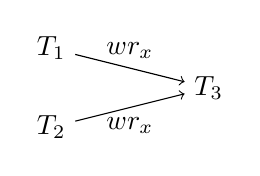
\begin{tikzpicture}[node distance=3cm]
\tikzstyle{tx}=[draw=none, fill=none]
\node[tx] (T1) at (0,0) {$T_1$};
\node[tx] (T2) at (0,-1) {$T_2$};
\node[tx] (T3) at (2,-.5) {$T_3$};

\draw[->] (T1) edge node[above]{$wr_x$} (T3);
\draw[->] (T2) edge node[below]{$wr_x$} (T3);
\end{tikzpicture}
\caption{DSG for Figure~\ref{fig:nici-history}.}
\label{fig:nici-dsg}
\end{figure}

\begin{definition}[Item Cut Isolation (I-CI)]
A system that provides Item Cut Isolation prohibits phenomenon N-I-CI.
\end{definition}

\begin{definition}[Predicate Cut Non-Isolation (N-P-CI)]
A history $H$ exhibits phenomenon N-I-CI if $DSG(H)$ contains a
transaction $T_i$ such that, for two predicate-based reads $p_k$,
$p_j$ in $P$ such that $p_k \subseteq p_j$ and $T_i$ directly
predicate-read-depends by $p_k$ on another transaction $T_l$, but
$T_i$ does not directly predicate-read-depend by $p_j$ on $T_l$.
\end{definition}

\begin{definition}[Predicate Cut Isolation (P-CI)]
A system that provides Predicate Cut Isolation prohibits phenomenon N-P-CI.
\end{definition}

\begin{definition}[Non-transactional Atomicity (N-TA)]
A history $H$ exhibits phenomenon N-TA if $DSG(H)$ contains a directed cycle
consisting of exactly one read-dependency edge by $x$ from $T_i$ to
$T_j$ and one anti-dependency edge by $y$ from $T_j$ to $T_i$ and
$T_i$'s corresponding read from $x$ does not precede its corresponding
read from $y$.
\end{definition}


\begin{figure}[H]
\begin{align*}
\small
T_1 &: w_x(1)~w_y(1)\\
T_2 &: w_x(2)~w_y(2)\\
T_3 &: r_x(2)~r_y(1)
\end{align*}
\caption{Example of \textit{N-TA} anomaly.}
\label{fig:nta-history}
\end{figure}

\begin{figure}[H]
\centering
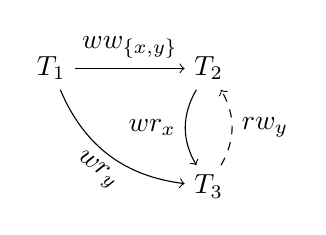
\begin{tikzpicture}[node distance=3cm]
\tikzstyle{tx}=[draw=none, fill=none]
\node[tx] (T1) at (0,0) {$T_1$};
\node[tx] (T2) at (2,0) {$T_2$};
\node[tx] (T3) at (2,-1.5) {$T_3$};

\draw[->] (T1) edge node[sloped, above]{$ww_{\{x, y\}}$} (T2);
\draw[->] (T1) edge [bend right] node[sloped, below]{$wr_y$} (T3);
\draw[->] (T2) edge [bend right] node[left]{$wr_x$} (T3);
\draw[dashed, ->] (T3) edge [bend right] node[right]{$rw_y$} (T2);
\end{tikzpicture}
\caption{DSG for Figure~\ref{fig:nta-history}.}
\label{fig:nta-dsg}
\end{figure}

\begin{definition}[Transactional Atomicity (TA)]
A system that provides transactional atomicity prohibits phenomenon
N-TA.
\end{definition}

\begin{definition}[Non-monotonic Reads (N-MR)]
A history $H$ exhibits phenomenon N-MR if $DSG(H)$ contains a directed cycle
consisting of a transitive session-dependency between transactions
$T_j$ and $T_i$ with an anti-dependency edge by $i$ from $T_j$ and a
read-dependency edge by $i$ into $T_i$.
\end{definition}

\begin{definition}[Monotonic Reads (MR)]
A system provides Monotonic Reads if it prohibits phenomenon N-MR.
\end{definition}


\begin{figure}[H]
\begin{align*}
\small
T_1 &: w_x(1)\\
T_2 &: w_x(2)\\
T_3 &: r_x(2)\\
T_4 &: r_x(1)
\end{align*}
\caption{Example of \textit{N-MR} violation when $w_x(1) \ll w_x(2)$ and $T_4$ directly session-depends on $T_3$.}
\label{fig:nmr-history}
\end{figure}

\begin{figure}[H]
\centering
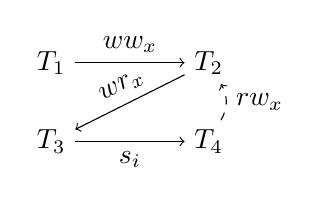
\begin{tikzpicture}[node distance=3cm]
\tikzstyle{tx}=[draw=none, fill=none]
\node[tx] (T1) at (0,0) {$T_1$};
\node[tx] (T2) at (2,0) {$T_2$};

\node[tx] (T3) at (0,-1) {$T_3$};
\node[tx] (T4) at (2,-1) {$T_4$};

\draw[->] (T1) edge node[above]{$ww_x$} (T2);
\draw[->] (T3) edge node[below]{$s_i$} (T4);

\draw[->] (T2) edge node[sloped, above]{$wr_x$} (T3);
%\draw[->] (T2) edge [bend right] node[left]{$wr_x$} (T4);
%\draw[->] (T1) edge [bend right]node[right]{$wr_x$} (T4);
\draw[dashed, ->] (T4) edge [bend right]node[right]{$rw_x$} (T2);
\end{tikzpicture}
\caption{DSG for Figure~\ref{fig:nmr-history}. $wr_x$ dependency from $T_1$ to $T_4$ omitted.} 
\label{fig:nmr-dsg}
\end{figure}

\begin{definition}[Non-monotonic Writes (N-MW)]
A history $H$ exhibits phenomenon N-MW if $DSG(H)$ contains a directed cycle
consisting of a transitive session-dependency between transactions
$T_j$ and $T_i$ and at least one write-dependency edge.
\end{definition}


\begin{figure}[H]
\begin{align*}
\small
T_1 &: w_x(1)\\
T_2 &: w_y(1)\\
T_3 &: r_y(1)~r_x(0)
\end{align*}
\caption{Example of \textit{N-MW} anomaly if $T_2$ directly session-depends on $T_1$.}
\label{fig:nmw-history}
\end{figure}

\begin{figure}[H]
\centering
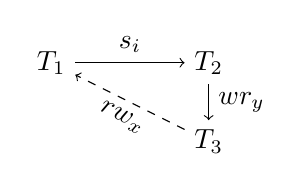
\begin{tikzpicture}[node distance=3cm]
\tikzstyle{tx}=[draw=none, fill=none]
\node[tx] (T1) at (0,0) {$T_1$};
\node[tx] (T2) at (2,0) {$T_2$};
\node[tx] (T3) at (2,-1) {$T_3$};

\draw[->] (T1) edge node[above]{$s_i$} (T2);
\draw[->] (T2) edge node[right]{$wr_y$} (T3);
\draw[->, dashed] (T3) edge node[below, sloped]{$rw_x$} (T1);
\end{tikzpicture}
\caption{DSG for Figure~\ref{fig:nmw-history}.}
\label{fig:nmw-dsg}
\end{figure}


\begin{definition}[Monotonic Writes (MW)]
A system provides Monotonic Writes if it prohibits phenomenon N-MW.
\end{definition}

\begin{definition}[Writes Do Not Follow Reads (N-WFR)]
A history $H$ exhibits phenomenon N-WFR if, in $DSG(H)$, for all
committed transactions $T_1$, $T_2$, $T_3$ such that $T_2$
write-depends on $T_1$ and $T_3$ write-depends on $T_2$, $T_3$ does
not directly anti-depend on $T_1$.
\end{definition}


\begin{figure}[H]
\begin{align*}
\small
T_1 &: w_x(1)\\
T_2 &: r_x(1) w_y(1)\\
T_3 &: r_y(1)~r_x(0)
\end{align*}
\caption{Example of \textit{N-WFR} anomaly.}
\label{fig:nwfr-history}
\end{figure}

\begin{figure}[H]
\centering
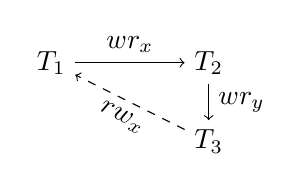
\begin{tikzpicture}[node distance=3cm]
\tikzstyle{tx}=[draw=none, fill=none]
\node[tx] (T1) at (0,0) {$T_1$};
\node[tx] (T2) at (2,0) {$T_2$};
\node[tx] (T3) at (2,-1) {$T_3$};

\draw[->] (T1) edge node[above]{$wr_x$} (T2);
\draw[->] (T2) edge node[right]{$wr_y$} (T3);
\draw[->, dashed] (T3) edge node[below, sloped]{$rw_x$} (T1);
\end{tikzpicture}
\caption{DSG for Figure~\ref{fig:nwfr-history}.}
\label{fig:nwfr-dsg}
\end{figure}

\begin{definition}[Writes Follow Reads (WFR)]
A system provides Writes Follow Reads if it prohibits phenomenon N-WFR.
\end{definition}

\begin{definition}[Not-Read Your Writes (N-RYW)]
A history $H$ exhibits phenomenon N-RYW if $DSG(H)$ contains a directed cycle
consisting of a transitive session-dependency between transactions
$T_j$ and $T_i$, at least one anti-dependency edge, and the remainder
anti-dependency or write-dependency edges.
\end{definition}


\begin{figure}[H]
\begin{align*}
\small
T_1 &: w_x(1)\\
T_2 &: r_x(0)\\
\end{align*}
\caption{Example of \textit{N-RYW} anomaly if $T_2$ directly session-depends on $T_1$.}
\label{fig:nryw-history}
\end{figure}

\begin{figure}[H]
\centering
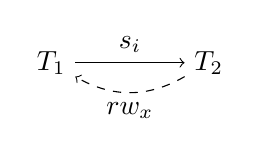
\begin{tikzpicture}[node distance=3cm]
\tikzstyle{tx}=[draw=none, fill=none]
\node[tx] (T1) at (0,0) {$T_1$};
\node[tx] (T2) at (2,0) {$T_2$};

\draw[->] (T1) edge node[above]{$s_i$} (T2);
\draw[dashed, ->] (T2) edge [bend left] node[below]{$rw_x$} (T1);
\end{tikzpicture}
\caption{DSG for Figure~\ref{fig:nwfr-history}.}
\label{fig:nryw-dsg}
\end{figure}

\begin{definition}[Read Your Writes (RYW)]
A system provides Read Your Writes if it prohibits phenomenon N-RYW.
\end{definition}

\begin{definition}[PRAM Consistency]
A system provides PRAM Consistency if it prohibits phenomenon N-MR,
N-MW, and N-RYW.
\end{definition}

\begin{definition}[Causal Consistency]
A system provides Causal Consistency if it provides PRAM Consistency
and prohibits phenomenon N-WFR.
\end{definition}

\begin{definition}[Lost Update]
A history $H$ exhibits phenomenon Lost if $DSG(H)$ contains a directed
cycle having one or more item-antidependency edges and all edges are
by the same data item $x$.
\label{def:lostupdate}
\end{definition}

\begin{definition}[Write Skew (Adya G2-item)]
A history $H$ exhibits phenomenon Write Skew if $DSG(H)$ contains a directed
cycle having one or more item-antidependency edges.
\end{definition}

For Snapshot Isolation, we depart from Adya's recency-based definition
(see Adya Section 4.3). Nonetheless, implementations of this
definition will still be unavailable due to reliance of preventing
Lost Update.

\begin{definition}[Snapshot Isolation]
A system that provides Snapshot Isolation prevents phenomena G0, G1a,
G1b, G1c, N-P-CI, N-TA, and Lost Update.
\end{definition}

For Repeatable Read, we return to Adya.

\begin{definition}[Repeatable Read]
A system that provides Repeatable Read Isolation prohibits phenomena
G0, G1a, G1b, G1c, and Write Skew.
\end{definition}

For definitions of safe, regular, and linearizable register semantics,
we refer the reader to Herlihy's textbook~\cite{herlihy-art}.

\section{Transactional Atomicity}

In our non-sticky TA algorithm, clients buffer their writes until
commit, sending the final write to each data item to each respective
server. Along with each write, clients attach a the transaction ID and
a list of all data items written to in the transaction, $L_v$. Upon
receiving a new write to item $d$, a server places the write into a
\texttt{pending} queue and notifies all other servers responsible for
a data item in $L_v$ that it has received a write to $d$ with the
respective transaction ID. Once a server receives acknowledgments with
appropriate transaction ID for all items in $L_v$, it moves the write
from \texttt{pending} to the \texttt{stable} database (which applies
the writes according to highest-ID-wins). Accordingly, all writes that
should be made atomic with a write in \texttt{stable} are guaranteed
to be present on their respective servers, either in \texttt{pending}
or \texttt{stable}. Given the possibility of internal aborts, writes
to \texttt{pending} may require 2 RTTs: one to check constraints and
one to execute the above (but these checks \textit{cannot} cause other
transactions to block, as would be the case in a two-phase
\textit{commit} protocol).

For reads, each client tracks which values it should read. It
maintains a mapping (vector) from data items to transaction IDs. Upon
transaction start, the client clears its mapping, and, when it
performs a read from a data item, it sends the server its current ID
for the item. If the client does not supply an ID, the server returns
the latest value from \texttt{stable}. If the ID is non-empty, the
server either returns the matching value from \texttt{pending} or a
value with higher ID from \texttt{pending}---along with $L_v$ for the
write. When the client receives a response, it updates its local
vector with $L_v$. Accordingly, even if transaction's writes to two
keys $x$ and $y$ are present on the replica for $x$'s \texttt{stable}
and the replica for $y$'s \texttt{pending}, a client's reads from $x$
then $y$ will return a transactionally atomic pair of values because
the replica for $y$ will know to check \texttt{pending}.


\begin{algorithm}[t!]
\newcommand{\myindent}{\hspace{-1em}}
\begin{addmargin}[-1em]{0em}% 1em left, 2em right

\begin{algorithmic}
\caption*{\textbf{Algorithm} HAT Transactional Atomicity}\vspace{.5em}
\State{\textit{\textbf{Shared Data Types}}\\\vspace{.5em}
\texttt{timestamp}: unique, per transaction identifier\\
$\texttt{write}:[\texttt{key:}k, \texttt{value}:v, \texttt{timestamp}:ts, \texttt{set<key>}:tx\_keys]$\\\hrulefill}\vspace{.5em}

  \State{\textbf{\textit{Server-side Data Structures and Methods}\\\vspace{.5em}
$\texttt{set<write>:pending}$\\
$\texttt{set<write>:good}$\\
$\texttt{map<timestamp, int>:acks}$}}\\

\Procedure{put}{\texttt{write}:$w$}
  \State \texttt{pending}.add($w$)
  \For{key $k_t \in w.tx\_keys$}
  \State \{all replicas for $sib$\}.notify($w.ts$)
  \EndFor
  
  \State \textit{asynchronously send $w$ to other replicas via anti-entropy}
  \State \Return

  \EndProcedure\vspace{.5em}

  \Procedure{notify}{\texttt{timestamp}:$ts$}
  \State \texttt{acks}.get($ts$).increment()
  \If{all \texttt{acks} received for all replicas for $ts$'s $tx\_keys$}
  \State \texttt{good}.add($w$)
  \State \texttt{pending}.remove($w$)  
  \EndIf  
  \EndProcedure\vspace{.5em}

  \Procedure{get}{\texttt{key}:$k$, \texttt{timestamp}:$ts_{required}$}
  \If{$ts_{required} = \bot$}
  \State \Return $w \in \texttt{good}$ s.t. $w.key = key$ with highest timestamp
  \ElsIf{$\exists~w \in \texttt{good}$ s.t. $w.key = key, w.ts \geq ts_{required}$}
  \State \Return $w$
  \Else
  \State \Return $w \in \texttt{pending}$ s.t. $w.key = key,  w.ts = ts_{required}$
  \EndIf
  \EndProcedure\\\vspace{-.5em}\hrulefill\vspace{.25em}

  \State{\textbf{\textit{Client-side Data Structures and Methods}\\\vspace{.5em}
$\texttt{int:cur\_txn}$\\
$\texttt{map<key, value>:write\_buffer}$\\
$\texttt{map<key, timestamp>:required}$}}\\


\Procedure{begin\_transaction}{}
  \State \texttt{cur\_txn} = \textit{new txn ID} \commentt{// (e.g., clientID+logicalClock)}
  \EndProcedure\vspace{.5em}

\Procedure{put}{\texttt{key:$k$}, \texttt{value:$v$}}
  \State \texttt{write\_buffer}.put($k$, $v$)
\EndProcedure\vspace{.5em}

\Procedure{get}{\texttt{key:$k$}}
  \If {$k \in \texttt{write\_buffer}$}
  \State \Return \texttt{write\_buffer}.get($k$) \commentt{// if we want per-TxN RYW}
  \EndIf

  \State $w\_{ret}$ = (available replica for $k$).get($k$, \texttt{required}.get($k$))
  \For {$(tx_{key} \in w_{ret}.tx\_keys$}
  \If {$w_{ret}.ts > \texttt{required}.get(tx_{key})$}
  \State $\texttt{required}$.put$(tx_{key}, w_{ret}.ts)$
  \EndIf
  \EndFor

  \State \Return $w\_{ret}.value$
\EndProcedure\vspace{.5em}


\Procedure{commit}{}
 \For{$(tx_{key}, v) \in \texttt{write\_buffer}$}
 \State $r$ = (available replica for $tx_{key}$)
 \State $r$.put($[tx_{key}, v, \texttt{cur\_txn}, \texttt{write\_buffer}.keys()]$)
 \EndFor
  \State \textsc{cleanup()}
\EndProcedure\vspace{.5em}


\Procedure{abort}{}
  \State \textsc{cleanup()}
\EndProcedure\vspace{.5em}


\Procedure{cleanup}{}
  \State \texttt{write\_buffer}.clear()
  \State \texttt{required\_map}.clear()
\EndProcedure\vspace{.5em}


\end{algorithmic}
\end{addmargin}
\end{algorithm}
